\chapter{Formulario de Distribuciones de Probabilidad}
\section{Conceptos y Fórmulas Generales}
\vspace{0.5em}
\begin{itemize}\setlength\itemsep{0.5em}
    \item \textbf{Función de Distribución Acumulada (FDC):} $F_X(x) = \mathbb{P}(X \le x)$. \\ Caso continuo: $F_X(x) = \int_{-\infty}^{x} f_X(t) \, dt$.
    \item \textbf{Esperanza Matemática:} $\displaystyle \mathbb{E}[X] = \sum_{x \in \mathcal{X}} x p_X(x)$ (discreto) o $\displaystyle \mathbb{E}[X] = \int_{-\infty}^{\infty} x f_X(x) \, dx$ (continuo).
    \item \textbf{Varianza:} $\text{Var}(X) = \mathbb{E}[(X - \mathbb{E}[X])^2] = \mathbb{E}[X^2] - (\mathbb{E}[X])^2$.
    \item \textbf{Función Generadora de Momentos (FGM):} $M_X(t) = \mathbb{E}[e^{tX}]$. Propiedad clave: $\mathbb{E}[X^n] = \frac{d^n}{dt^n}M_X(t)\Big|_{t=0}$.
    \item \textbf{Teorema de Bayes:} $\displaystyle \mathbb{P}(A_i\mid B) = \frac{\mathbb{P}(B \mid A_i)\, \mathbb{P}(A_i)}{\sum_j \mathbb{P}(B \mid A_j)\, \mathbb{P}(A_j)}$.
\end{itemize}
\newpage
\section{Distribuciones Discretas}
\subsection*{Distribución Bernoulli, $X \sim \text{Bern}(p)$}
Sea $X$ una variable aleatoria que modeliza un único ensayo dicotómico: éxito ($X=1$) con probabilidad $p \in (0,1)$ y fracaso ($X=0$) con probabilidad $q = 1-p$.

\vspace{0.8em}
\noindent
\begin{minipage}[c]{0.45\textwidth}
    \textbf{Propiedades:}
    \begin{itemize}\setlength\itemsep{0.3em}
        \item \textbf{Soporte:} $\mathcal{X} = \{0, 1\}$
        \item \textbf{FMP:} $p_X(x) = p^x (1-p)^{1-x}$
        \item $\mathbb{E}[X] = p$
        \item $\text{Var}(X) = p(1-p)$
        \item \textbf{FGM:} $M_X(t) = (1-p) + p e^t$
    \end{itemize}
\end{minipage}%
\hfill
\begin{minipage}[c]{0.5\textwidth}
    \begin{center}
    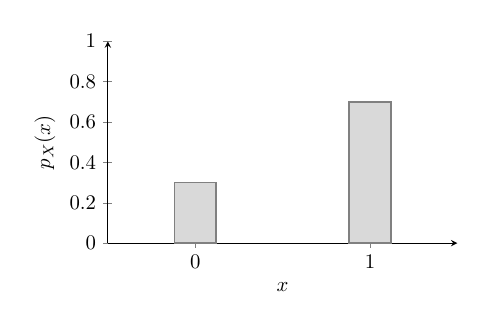
\begin{tikzpicture}[scale=0.75]
        \begin{axis}[
            ybar,
            ymin=0, ymax=1, xmin=-0.5, xmax=1.5,
            xtick={0, 1},
            ylabel={$p_X(x)$}, xlabel={$x$},
            bar width=20pt,
            height=5cm, width=7.5cm,
            axis lines=left
        ]
            \addplot[fill=gray!30, draw=gray, thick] coordinates {(0,0.3) (1,0.7)};
        \end{axis}
    \end{tikzpicture}
    \end{center}
\end{minipage}

\vspace{1.5em}

\subsection*{Distribución Binomial, $X \sim \text{Bin}(n, p)$}
Número de éxitos en $n$ ensayos independientes e idénticamente distribuidos, donde cada ensayo es $\text{Bern}(p)$.

\vspace{0.8em}
\noindent
\begin{minipage}[c]{0.45\textwidth}
    \textbf{Propiedades:}
    \begin{itemize}\setlength\itemsep{0.3em}
        \item \textbf{Soporte:} $\mathcal{X} = \{0, 1, \dots, n\}$
        \item \textbf{FMP:} $p_X(k) = \binom{n}{k} p^k (1-p)^{n-k}$
        \item $\mathbb{E}[X] = np$
        \item $\text{Var}(X) = np(1-p)$
        \item \textbf{FGM:} $M_X(t) = (1 - p + p e^t)^n$
    \end{itemize}
\end{minipage}%
\hfill
\begin{minipage}[c]{0.5\textwidth}
    \begin{center}
    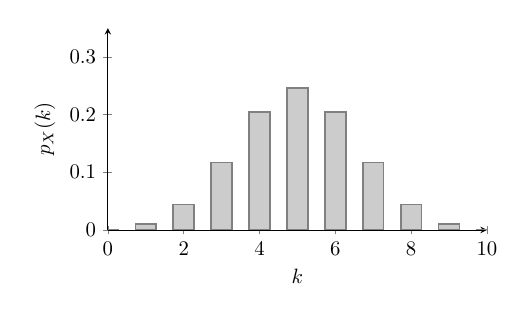
\begin{tikzpicture}[scale=0.75]
        \begin{axis}[
            ybar,
            ymin=0, ymax=0.35,
            xlabel={$k$}, ylabel={$p_X(k)$},
            bar width=10pt,
            height=5cm, width=8cm,
            axis lines=left
        ]
            \addplot[fill=gray!40, draw=gray, thick] coordinates {
                (0,0.001) (1,0.010) (2,0.044) (3,0.117) 
                (4,0.205) (5,0.246) (6,0.205) (7,0.117) 
                (8,0.044) (9,0.010) (10,0.001)
            };
        \end{axis}
    \end{tikzpicture}
    \end{center}
\end{minipage}

\vspace{1.5em}

\subsection*{Distribución Poisson, $X \sim \text{Poisson}(\lambda)$}
Modela el número de ocurrencias de un suceso en un intervalo continuo a una tasa media constante $\lambda > 0$.

\vspace{0.8em}
\noindent
\begin{minipage}[c]{0.45\textwidth}
    \textbf{Propiedades:}
    \begin{itemize}\setlength\itemsep{0.3em}
        \item \textbf{Soporte:} $\mathcal{X} = \{0, 1, 2, \dots\}$
        \item \textbf{FMP:} $p_X(k) = \frac{\lambda^k e^{-\lambda}}{k!}$
        \item $\mathbb{E}[X] = \lambda$
        \item $\text{Var}(X) = \lambda$
        \item \textbf{FGM:} $M_X(t) = \exp\left(\lambda(e^t - 1)\right)$
    \end{itemize}
\end{minipage}%
\hfill
\begin{minipage}[c]{0.5\textwidth}
    \begin{center}
    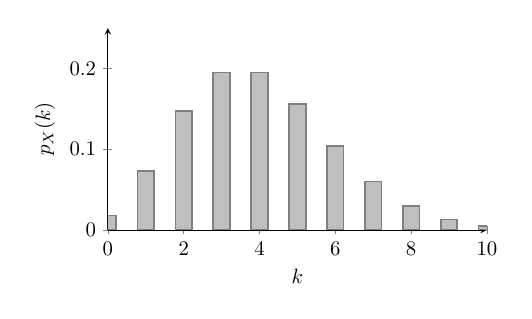
\begin{tikzpicture}[scale=0.75]
        \begin{axis}[
            ybar,
            ymin=0, ymax=0.25,
            xlabel={$k$}, ylabel={$p_X(k)$},
            bar width=8pt,
            height=5cm, width=8cm,
            axis lines=left
        ]
            \addplot[fill=gray!50, draw=gray, thick] coordinates {
                (0,0.018) (1,0.073) (2,0.147) (3,0.195) 
                (4,0.195) (5,0.156) (6,0.104) (7,0.060) 
                (8,0.030) (9,0.013) (10,0.005)
            };
        \end{axis}
    \end{tikzpicture}
    \end{center}
\end{minipage}

\newpage

\section{Distribuciones Continuas}
\vspace{0.5em}

\subsection*{Distribución Uniforme Continua, $X \sim \mathcal{U}(a, b)$}
Variable que asigna una densidad equiprobable en el intervalo real $[a, b]$.

\vspace{0.8em}
\noindent
\begin{minipage}[c]{0.45\textwidth}
    \textbf{Propiedades:}
    \begin{itemize}\setlength\itemsep{0.3em}
        \item \textbf{Soporte:} $\mathcal{X} = [a, b]$
        \item \textbf{FDP:} $f_X(x) = \frac{1}{b-a}$
        \item \textbf{FDC:} $F_X(x) = \frac{x-a}{b-a}$
        \item $\mathbb{E}[X] = \frac{a+b}{2}$
        \item $\text{Var}(X) = \frac{(b-a)^2}{12}$
    \end{itemize}
\end{minipage}%
\hfill
\begin{minipage}[c]{0.5\textwidth}
    \begin{center}
    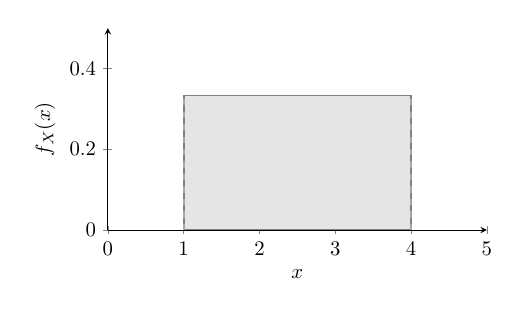
\begin{tikzpicture}[scale=0.75]
        \begin{axis}[
            ymin=0, ymax=0.5, xmin=0, xmax=5,
            xlabel={$x$}, ylabel={$f_X(x)$},
            height=5cm, width=8cm,
            axis lines=left
        ]
            \addplot[thick, gray, fill=gray!20] coordinates {(1,0) (1,0.333) (4,0.333) (4,0)} \closedcycle;
            \addplot[dashed, gray!70, thick] coordinates {(1,0) (1,0.333)};
            \addplot[dashed, gray!70, thick] coordinates {(4,0) (4,0.333)};
        \end{axis}
    \end{tikzpicture}
    \end{center}
\end{minipage}

\vspace{1.5em}

\subsection*{Distribución Normal, $X \sim \mathcal{N}(\mu, \sigma^2)$}
Piedra angular de la inferencia estadística (por el teorema del Límite Central).

\vspace{0.8em}
\noindent
\begin{minipage}[c]{0.45\textwidth}
    \textbf{Propiedades:}
    \begin{itemize}\setlength\itemsep{0.3em}
        \item \textbf{Soporte:} $\mathcal{X} = \mathbb{R}$
        \item \textbf{FDP:} $f_X(x) = \frac{1}{\sigma \sqrt{2\pi}} e^{-\frac{(x-\mu)^2}{2\sigma^2}}$
        \item $\mathbb{E}[X] = \mu$
        \item $\text{Var}(X) = \sigma^2$
        \item \textbf{FGM:} $M_X(t) = \exp\left( \mu t + \frac{\sigma^2 t^2}{2} \right)$
    \end{itemize}
\end{minipage}%
\hfill
\begin{minipage}[c]{0.5\textwidth}
    \begin{center}
    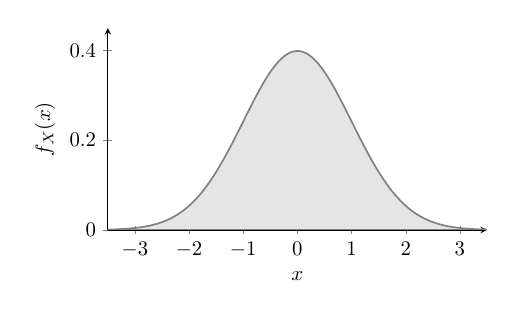
\begin{tikzpicture}[scale=0.75]
        \begin{axis}[
            no markers, domain=-3.5:3.5, samples=150,
            axis lines=left, xlabel={$x$}, ylabel={$f_X(x)$},
            height=5cm, width=8cm,
            ymin=0, ymax=0.45
        ]
            \addplot[thick, gray, fill=gray!20, smooth] {1/sqrt(2*pi)*exp(-x^2/2)} \closedcycle;
        \end{axis}
    \end{tikzpicture}
    \end{center}
\end{minipage}

\vspace{1.5em}

\subsection*{Distribución Exponencial, $X \sim \text{Exp}(\lambda)$}
Modela el tiempo transcurrido entre eventos en un proceso de Poisson con tasa $\lambda > 0$.

\vspace{0.8em}
\noindent
\begin{minipage}[c]{0.45\textwidth}
    \textbf{Propiedades:}
    \begin{itemize}\setlength\itemsep{0.3em}
        \item \textbf{Soporte:} $\mathcal{X} = [0, \infty)$
        \item \textbf{FDP:} $f_X(x) = \lambda e^{-\lambda x}$
        \item \textbf{FDC:} $F_X(x) = 1 - e^{-\lambda x}$
        \item $\mathbb{E}[X] = \frac{1}{\lambda}$
        \item $\text{Var}(X) = \frac{1}{\lambda^2}$
    \end{itemize}
\end{minipage}%
\hfill
\begin{minipage}[c]{0.5\textwidth}
    \begin{center}
    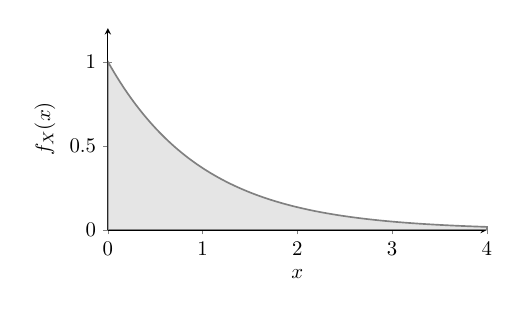
\begin{tikzpicture}[scale=0.75]
        \begin{axis}[
            no markers, domain=0:4, samples=100,
            axis lines=left, xlabel={$x$}, ylabel={$f_X(x)$},
            height=5cm, width=8cm,
            ymin=0, ymax=1.2
        ]
            \addplot[thick, gray, fill=gray!20, smooth] {1*exp(-1*x)} \closedcycle;
        \end{axis}
    \end{tikzpicture}
    \end{center}
\end{minipage}

\vspace{1.5em}

\subsection*{Distribución Gamma, $X \sim \Gamma(\alpha, \lambda)$}
Tiempo de espera hasta el $\alpha$-ésimo evento en un proceso de Poisson con tasa $\lambda > 0$.

\vspace{0.8em}
\noindent
\begin{minipage}[c]{0.45\textwidth}
    \textbf{Propiedades:}
    \begin{itemize}\setlength\itemsep{0.3em}
        \item \textbf{Soporte:} $\mathcal{X} = (0, \infty)$
        \item \textbf{FDP:} $f_X(x) = \frac{\lambda^\alpha}{\Gamma(\alpha)} x^{\alpha-1} e^{-\lambda x}$
        \item $\mathbb{E}[X] = \frac{\alpha}{\lambda}$
        \item $\text{Var}(X) = \frac{\alpha}{\lambda^2}$
        \item \textbf{FGM:} $M_X(t) = \left(\frac{\lambda}{\lambda - t}\right)^\alpha$
    \end{itemize}
\end{minipage}%
\hfill
\begin{minipage}[c]{0.5\textwidth}
    \begin{center}
    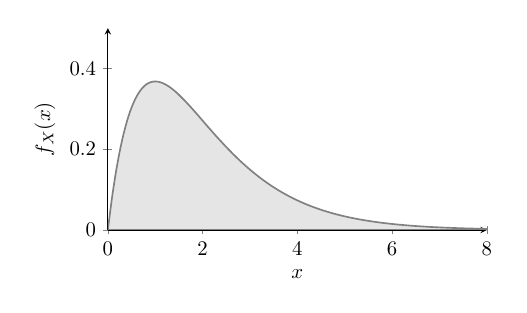
\begin{tikzpicture}[scale=0.75]
        \begin{axis}[
            no markers, domain=0:8, samples=100,
            axis lines=left, xlabel={$x$}, ylabel={$f_X(x)$},
            height=5cm, width=8cm,
            ymin=0, ymax=0.5
        ]
            \addplot[thick, gray, fill=gray!20, smooth] {x*exp(-x)} \closedcycle;
        \end{axis}
    \end{tikzpicture}
    \end{center}
\end{minipage}

\subsection*{Distribución Beta, $X \sim \text{Beta}(\alpha, \beta)$}
Útil para modelar proposicionorciones y probabilidades continuas acotadas en inferencia bayesiana.

\vspace{0.8em}
\noindent
\begin{minipage}[c]{0.45\textwidth}
    \textbf{Propiedades:}
    \begin{itemize}\setlength\itemsep{0.3em}
        \item \textbf{Soporte:} $\mathcal{X} = (0, 1)$
        \item \textbf{FDP:} $f_X(x) = \frac{x^{\alpha-1} (1-x)^{\beta-1}}{\text{B}(\alpha, \beta)}$
        \item $\mathbb{E}[X] = \frac{\alpha}{\alpha+\beta}$
        \item $\text{Var}(X) = \frac{\alpha\beta}{(\alpha+\beta)^2(\alpha+\beta+1)}$
    \end{itemize}
\end{minipage}%
\hfill
\begin{minipage}[c]{0.5\textwidth}
    \begin{center}
    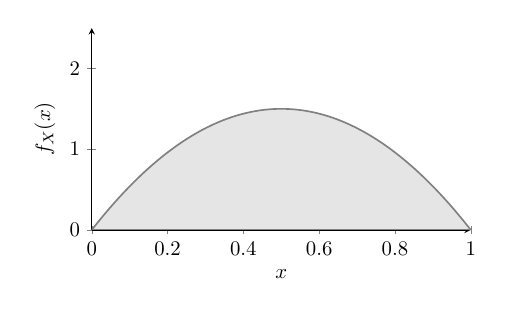
\begin{tikzpicture}[scale=0.75]
        \begin{axis}[
            no markers, domain=0:1, samples=150,
            axis lines=left, xlabel={$x$}, ylabel={$f_X(x)$},
            height=5cm, width=8cm,
            ymin=0, ymax=2.5
        ]
            \addplot[thick, gray, fill=gray!20, smooth] {6*x*(1-x)} \closedcycle;
        \end{axis}
    \end{tikzpicture}
    \end{center}
\end{minipage}

\vspace{1.5em}

\subsection*{Distribución Chi-cuadrado, $X \sim \chi^2_k$}
Suma de $k$ variables aleatorias $\mathcal{N}(0,1)$ al cuadrado. Equivale a una distribución $\Gamma(k/2, 1/2)$.

\vspace{0.8em}
\noindent
\begin{minipage}[c]{0.45\textwidth}
    \textbf{Propiedades:}
    \begin{itemize}\setlength\itemsep{0.3em}
        \item \textbf{Soporte:} $\mathcal{X} = (0, \infty)$
        \item \textbf{FDP:} $f_X(x) = \frac{x^{k/2-1} e^{-x/2}}{2^{k/2}\Gamma(k/2)}$
        \item $\mathbb{E}[X] = k$
        \item $\text{Var}(X) = 2k$
        \item \textbf{FGM:} $M_X(t) = (1 - 2t)^{-k/2}$
    \end{itemize}
\end{minipage}%
\hfill
\begin{minipage}[c]{0.5\textwidth}
    \begin{center}
    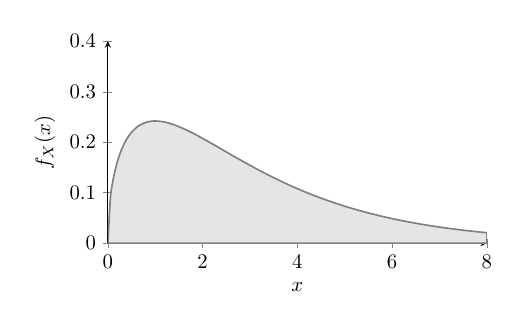
\begin{tikzpicture}[scale=0.75]
        \begin{axis}[
            no markers, domain=0:8, samples=150,
            axis lines=left, xlabel={$x$}, ylabel={$f_X(x)$},
            height=5cm, width=8cm,
            ymin=0, ymax=0.4
        ]
            \addplot[thick, gray, fill=gray!20, smooth] {0.3989 * x^(0.5) * exp(-x/2)} \closedcycle;
        \end{axis}
    \end{tikzpicture}
    \end{center}
\end{minipage}

\vspace{2.5em}

\section{Distribuciones Derivadas en la Inferencia Muestral}
\vspace{0.8em}

\noindent A continuación se presentan las distribuciones fundamentales derivadas de la normal, esenciales en la teorema de estimación y el contraste de hipótesis paramétricas:

\vspace{1.5em}

\begin{center}
\renewcommand{\arraystretch}{1.8}
\begin{tabular}{lcccc}
    \toprule
    \textbf{Distribución} & \textbf{Definición Estocástica} & \textbf{Soporte} $\mathcal{X}$ & $\mathbb{E}[X]$ & $\text{Var}(X)$ \\
    \midrule
    \textbf{Chi-cuadrado} $\chi^2_k$ & $\sum_{i=1}^k Z_i^2$, con $Z_i \sim \mathcal{N}(0,1)$ i.i.d. & $[0, \infty)$ & $k$ & $2k$ \\
    \textbf{t de Student} $t_\nu$ & $\frac{Z}{\sqrt{V/\nu}}$, con $Z \sim \mathcal{N}(0,1), V \sim \chi^2_\nu$ & $(-\infty, \infty)$ & $0 \;\; (\nu > 1)$ & $\frac{\nu}{\nu-2} \;\; (\nu > 2)$ \\
    \textbf{F de Snedecor} $F_{d_1, d_2}$ & $\frac{U_1/d_1}{U_2/d_2}$, con $U_1 \sim \chi^2_{d_1}, U_2 \sim \chi^2_{d_2}$ & $[0, \infty)$ & $\frac{d_2}{d_2-2} \;\; (d_2 > 2)$ & Var. anal. $(d_2 > 4)$ \\
    \bottomrule
\end{tabular}
\end{center}

\vspace{1.5em}

\section*{V. Teorema de Muestras y Estimación Puntual}
\vspace{1em}

\noindent \textit{Definición} \textbf{(Muestra Aleatoria)}. Un vector aleatorio $(X_1, \dots, X_n)$ cuyas componentes son variables aleatorias independientes e idénticamente distribuidas (i.i.d.) con función de distribución común $F$.

\begin{itemize}
    \item \textbf{Estimador:} Toda variable aleatoria $\Theta_n = T(X_1, \dots, X_n)$ estadística que aproxima un parámetro desconocido $\theta$.
    \item \textbf{Sesgo:} $\bar{B}_n = \mathbb{E}[\Theta_n] - \theta$. Si $\bar{B}_n = 0$, el estimador se denomina \textit{insesgado}.
    \item \textbf{Error Cuadrático Medio (ECM):} $\text{ECM}(\Theta_n) = \mathbb{E}[(\Theta_n - \theta)^2] = \text{Var}(\Theta_n) + (\bar{B}_n)^2$.
    \item \textbf{Consistencia:} $\Theta_n$ es consistente si converge en probabilidad a $\theta$: $\Theta_n \xrightarrow{\mathbb{P}} \theta$. Una condición suficiente (consistencia en media cuadrática) es que $\lim_{n\to\infty} \text{Var}(\Theta_n) = 0$ y $\lim_{n\to\infty} \bar{B}_n = 0$.
\end{itemize}

\vspace{0.5em}

\noindent \textit{Estadísticos} \textbf{(Estadísticos Muestrales Fundamentales)}.

\begin{multicols}{2}
\begin{itemize}
    \item \textbf{Media Muestral:} 
    $$ \overline{X}_n = \frac{1}{n} \sum_{i=1}^n X_i $$
    Insesgada ($\mathbb{E}[\overline{X}_n] = \mu$), varianza $\text{Var}(\overline{X}_n) = \frac{\sigma^2}{n}$, y consistente a $\mu$.
    
    \item \textbf{Cuasi-varianza Muestral:} 
    $$ S_n^2 = \frac{1}{n-1} \sum_{i=1}^n (X_i - \overline{X}_n)^2 $$
    Estimador insesgado de la varianza poblacional ($\mathbb{E}[S_n^2] = \sigma^2$) y consistente ($S_n^2 \xrightarrow{\mathbb{P}} \sigma^2$).
\end{itemize}
\end{multicols}

\vspace{0.5em}

\noindent \textbf{Teorema de Fisher para Poblaciones Normales}. Sea $X_1, \dots, X_n$ una muestra aleatoria tal que sus componentes son normales idénticamente distribuidas, $X_i \sim \mathcal{N}(\mu, \sigma^2)$. Entonces se verifica que:
\begin{enumerate}
    \item La media muestral es normal: $\overline{X}_n \sim \mathcal{N}\left(\mu, \frac{\sigma^2}{n}\right)$.
    \item La media muestral y la cuasi-varianza muestral son variables aleatorias estrictamente independientes: $\overline{X}_n \perp S_n^2$.
    \item La distribución de la varianza muestral escalada sigue una distribución chi-cuadrado con $n-1$ grados de libertad: 
    $$ \frac{(n-1)S_n^2}{\sigma^2} = \frac{1}{\sigma^2} \sum_{i=1}^n (X_i - \overline{X}_n)^2 \sim \chi^2_{n-1} $$
\end{enumerate}

\section*{V. Transformaciones y Función Característica}

\section*{Definición}{Función Característica} La función característica de una v.a. $X$ es $\phi_X(s) = \mathbb{E}[e^{isX}]$. En el caso continuo es la transformada de Fourier de la densidad: $\phi(s) = \int_{-\infty}^{\infty} e^{isx} f_X(x) dx$.

\begin{teorema}[Suma de Variables Independientes]
Si $(X_1, \dots, X_n)$ son independientes, la función característica de la suma $Y = X_1 + \dots + X_n$ es el producto $\phi_Y(s) = \phi_{X_1}(s) \dots \phi_{X_n}(s)$.
\end{teorema}

\begin{proposicion}[Transformación Unidimensional]
Sea $X$ continua con densidad $f_X$ y sea $Y = T(X)$ donde $T$ es estrictamente monótona y $C^1$. Su inversa es $h = T^{-1}$. La densidad de $Y$ es $f_Y(y) = f_X(h(y)) \left| h'(y) \right|$.
\end{proposicion}

\section*{VI. teoremas Límite y Desigualdades}

\begin{teorema}[Desigualdad de Markov]
Si $\varphi(x) > 0$ es estrictamente creciente para $x \neq 0$, entonces $\mathbb{P}(|X| \ge M) \le \frac{\mathbb{E}[\varphi(X)]}{\varphi(M)}$.
\end{teorema}

\begin{teorema}[Desigualdad de Chebyshev]
Para la media $\mu$ y varianza $Var(X)$: $\mathbb{P}(|X - \mu| \ge M) \le \frac{Var(X)}{M^2}$.
\end{teorema}

\section*{Definición}{Modos de Convergencia} 
\begin{itemize}
    \item \textbf{Casi Seguro (c.s.):} $X_n \xrightarrow{c.s.} X_\infty \iff X_n(\omega) \to X_\infty(\omega)$ salvo en un conjunto nulo.
    \item \textbf{En Probabilidad ($\mathbb{P}$):} $\lim_{n\to\infty} \mathbb{P}(|X_n - X_\infty| \ge \epsilon) = 0$.
    \item \textbf{En Media Cuadrática ($L_2$):} $\lim_{n\to\infty} \mathbb{E}[|X_n - X_\infty|^2] = 0$.
    \item \textbf{En Distribución ($D$):} $\lim_{n\to\infty} F_{X_n}(x) = F_{X_\infty}(x)$.
\end{itemize}
Relaciones: Convergencia en $L_2$ implica convergencia en probabilidad. Convergencia en probabilidad implica convergencia en distribución. Convergencia casi seguro implica convergencia en probabilidad.

\begin{teorema}[Leyes de los Grandes Números y TCL]
Para una sucesión de variables $(X_n)$ independientes e idénticamente distribuidas (i.i.d.) con media $\mu$ y varianza $\sigma^2$ finitas:
\begin{itemize}
    \item \textbf{Ley Débil:} La media muestral $M_n = \frac{1}{n}\sum X_i$ converge en probabilidad a la esperanza: $M_n \xrightarrow{\mathbb{P}} \mu$.
    \item \textbf{Ley Fuerte:} $M_n \xrightarrow{c.s.} \mu$.
    \item \textbf{teorema Central del Límite (TCL):} $\frac{X_1 + \dots + X_n - n\mu}{\sigma\sqrt{n}} \xrightarrow{D} \mathcal{N}(0,1)$.
\end{itemize}
\end{teorema}

\section*{VII. Teorema de Muestras y Estimadores}

\section*{Definición}{Muestra y Estimador} Una muestra estadística es un vector $(X_1, \dots, X_n)$ donde $X_i$ son i.i.d. Un estimador es una v.a. $\Theta_n = T(X_1, \dots, X_n)$ que no depende de parámetros desconocidos.

\section*{Definición}{propiedades de un Estimador} 
\begin{itemize}
    \item \textbf{Sesgo:} $\bar{B}_n = \mathbb{E}[\Theta_n] - \theta$. Si es $0$, el estimador es \textbf{insesgado}.
    \item \textbf{Error Cuadrático Medio (ECM):} $\mathbb{E}[(\Theta_n - \theta)^2] = Var(\Theta_n) + (\bar{B}_n)^2$.
    \item \textbf{Consistencia:} $\Theta_n$ converge en probabilidad a $\theta$ ($\Theta_n \xrightarrow{\mathbb{P}} \theta$). Si un estimador es asintóticamente insesgado y su varianza tiende a 0, es consistente.
\end{itemize}

\begin{proposicion}[Media y Cuasi-Varianza Muestral]
La media muestral $\overline{X}_n = \frac{1}{n}\sum_{i=1}^n X_i$ es un estimador insesgado de $\mu$ con varianza $Var(\overline{X}_n) = \sigma^2/n$. La cuasi-varianza muestral $S_n^2 = \frac{1}{n-1}\sum_{i=1}^n (X_i - \overline{X}_n)^2$ es un estimador insesgado de la varianza $\sigma^2$.
\end{proposicion}

\begin{teorema}[teorema de Fisher]
Si la muestra proviene de una normal $X_i \sim \mathcal{N}(\mu, \sigma^2)$:
\begin{enumerate}
    \item $\overline{X}_n \sim \mathcal{N}(\mu, \sigma^2/n)$.
    \item $\overline{X}_n$ y $S_n^2$ son variables aleatorias independientes.
    \item $\frac{(n-1)S_n^2}{\sigma^2} \sim \chi^2_{n-1}$.
\end{enumerate}
\end{teorema}